\section{Tests et recettage}
Réaliser des tests pour l'application permet entre autres de ne pas perdre certaines fonctionnalités à cause d'un développement annexe, cela permet de vérifier constamment la disponibilité de celles-ci. Nous avons réalisé plusieurs séries de tests à plusieurs niveaux différents.  

\subsection{Cahier de recette}

Nous avons fait un cahier de recette sous forme de fichier Excel (\ref{Exemple d'un cahier de recettes (landing page)}). C'est ici que nous avons regroupé la majeure partie des features de l'application, les soucis de performance, les éventuels dysfonctionnements ou encore les fautes d'orthographe ou de traduction. Nous avons aussi réalisé manuellement le test de nos fonctionnalités (comme un utilisateur aurait pu le réaliser). C'est une pratique que nous avons pu voir en entreprise, surtout lors de la recherche à la reproduction d'un dysfonctionnement. Ce fut, tout au long de notre projet, un réel cahier de bord, facilitant ainsi la visualisation des tâches effectuées, ou de ce qu'il nous restait à faire.

\subsection{Tests unitaires}

Tout d'abord, les tests unitaires. Ce sont des test qui permettent de vérifier le bon fonctionnement d'une partie précise et définie de notre plateforme, comme par exemple la bonne traduction de celle-ci au moment du changement de langue, ou les tests de conversion de miles en kilomètres. Pour cela, nous avons décidé de mettre en place Jest: c'est un framework de test JavaScript. Nous l'avons couplé à Babel afin de définir au mieux sa scope d'utilisation, comme les fichiers à ne pas transpiler.

\subsection{Tests d'implémentation}

A la fin de chaque feature, on effectue des tests d'implémentation afin de savoir si en plus des features testées individuellement, ces dernières fonctionnent bien entre-elles et celles pré-existantes.

\subsection{Tests E2E}
Les tests E2E consistent à vérifier que le visiteur puisse parcourir les principaux scénarios d’utilisation de l’application. Pour se faire, nous avons configuré "puppeteer" afin de lancer automatiquement une instance headless de chromium (sans interface graphique) pour qu'il puisse tester certaines fonctionnalités. De plus, des tests de non-régression ont été mis en place afin de vérifier, en comparant avec un "snapshot" du resultat attendu, le bon fonctionnement des pages. Un "snapshot" est un fichier où l'entièreté du contenu d'une certaine page est enregistré en format JSON.

\subsection{Validations}

Chaque table de notre base de données est strictement définie avec des patterns de validation de schéma. Cela permet d'être sûr qu'un format respecte les attentes avant d'insérer un document dans la base de données. --> \ref{Exemple d'un schéma de validation (Drivers)}

\subsection{Tests GitHub Actions}

GitHub Actions constitue une sécurité supplémentaire avant un merge. En effet, à chaque commit, des tests automatisés se lancent afin de tester la mise en forme du code (avec eslint et prettier). Ces tests sont fait côté back-end et côté front-end.

\begin{figure}[th]
\centering
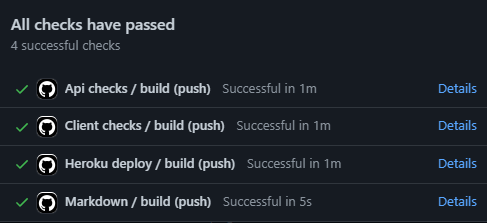
\includegraphics{medias/githubChecks.png}
\decoRule
\caption{Checkmark de Github Actions}
\end{figure}
